\section{AP checks and setting up}


These are checks that a Lead-Operator is required to do before including antenna positioners to be used in a subarray. 
\subsection{ Motion Profilers}

A profiler is needed because the servo loops are high gain loops; large position steps in 
a high gain system would inevitably lead to large overshoots. The profiler smoothens both the velocity and the acceleration profile. It ensures that the position controller is fed with small position increments only. It also provides velocity and acceleration feed forwards. The acceleration feed forward is enabled only in case of transitions between trajectories. Profiler handling is done automatically by the ACU. External commands from ACU or CAM may include any size of position steps within the operating range.

\subsection{To check if profilers are on or off}
It is required that profiles are always enabled on the AP at all times. But it is advisable that operators check the status of the profilers from time to time. 
\begin{lstlisting}[style=DOS, tabsize=4]
ssh kat@obs.mkat.karoo.kat.ac.za
Ipython
Import katuilib
configure_cam('camcam', 'all')
cam.print_sensors('profiler')

\end{lstlisting}

Switch profilers off
\begin{lstlisting}[style=DOS]
cam.m0XX.req.ap_enable_motion_profiler('elev', 0)
cam.m0XX.req.ap_enable_motion_profiler('azim', 0)
\end{lstlisting}

Switch profilers on
\begin{lstlisting}[style=DOS]
cam.m0XX.req.ap_enable_motion_profiler('elev', 1)
cam.m0XX.req.ap_enable_motion_profiler('azim', 1)
\end{lstlisting}
\subsection{ AP Point Error Tiltmeters}
The tiltmeter measures the the tilt of the antenna tower and by using a tiltmeter, pointing errors due to non-orthogonality of the azimuth axis and deformations of the azimuth structure because of temperature and constant wind can be compensated to a large extent [TBD]. The tiltmeter shall always be enabled.  The status of the tiltmeter can be checked from the ipython session. In the obs  machine do the following:
\begin{lstlisting}[style=DOS]
ipython
import katuilib
configure_cam('camcam',all)
\end{lstlisting}
Check the status of the point error tiltmeter sensor
\begin{lstlisting}[style=DOS]
cam.print_sensors('point_error_tiltmeter')
\end{lstlisting}
Enable the tiltmeter sensor
\begin{lstlisting}[style=DOS]
cam.m00X.req.ap_enable_point_error_tiltmeter(1)
\end{lstlisting}
The output will be as follows
\begin{lstlisting}[style=DOS]
!ap-enable-point-error-tiltmeter ok
\end{lstlisting}
Enable  tiltmeter sensor to all antennas
\begin{lstlisting}[style=DOS]

cam.ants.req.ap_enable_point_error_tiltmeter(1)
\end{lstlisting}
Disable the tiltmeter sensor
\begin{lstlisting}[style=DOS]
cam.m00X.req.ap_enable_point_error_tiltmeter(0)
\end{lstlisting}
The output will be as follows
\begin{lstlisting}[style=DOS]
!ap-enable-point-error-tiltmeter ok
\end{lstlisting}
\subsection{ Reporting AP Struct Tilt x/y  in error}
The risk caused by running observations with struct tilt errors will result in bad pointing offsets. 

Check status of the struct Tilt sensors in the GUI as follows: 
\begin{lstlisting}[style=DOS]
ap.struct-tilt-x  	error 	2019-07-12 14:59:06
ap.struct-tilt-y  	error 	2019-07-12 14:59:16-190.64
\end{lstlisting}
When reporting this error include the following in the JIRA to determine the course and action.

Check the  ap temp - plot sensorgraph
Check ap motion - plot azim and elev actual sensors
Is x/y tilt getting larger(correction value)? (Plot struct tilt x/y on sensorgraph)
Or is it a sudden jump to error? 
Checking these trends below will answer the question as to whether this is a matter of calibrating with correct values or is it a structural problem or not.
Report the JIRA to site AP teachnicians
\subsection{ SE tilt sensor measurements observations }
The purpose of the tilt measurements is to look at calibration tilt sensors and also to calculate tilt sensor offset parameters and compare these with set values. From a single test the calculated tilt sensor parameters did not match that closely to the set values. We were hoping to take many measurements so that we could see from the average of a number of low wind measurements if the calculated value matched the set values, especially for receptors where the calibration had recently been checked.   The next step was going to be to get to a point whereby we could automatically write the calculated values to the ACU to update the values. We have not reached that point yet.

\section{Receiver Checks and Setting Up }

\subsection{Positioning the Receiver Indexer}
Receiver Indexer (RI) carousel has four defined positions for each of the receivers it hosts. By selecting the frequency band on CAM’s  GUI during building of a subarray you are selecting a receiver position mounted on the indexer. Currently we are using L-band and UHF-band for observations and S-band is still being integrated. The raw angles for receivers when they are indexed are:
\begin{itemize}
	\item{} L band = 40deg
	\item{} X band = 80deg
	\item{} U band = 120deg
	\item{} S band = 0deg
\end{itemize}
There is no X band receiver installed and X-band position is used for parking antennas for the flight arrival and departure on site. 
In order to index the receiver manually to be used for the observation, on the obs machine obs.mkat.karoo.kat.ac.za,  run:	
\begin{lstlisting}[style=DOS]
ipython
Import katuilib
configure_cam('camcam', 'all')
cam.m0xx.req.mode('STOP') 
cam.m0xx.req.select_band('l', timeout=60)   
cam.m0xx.req.ap_set_indexer_position('l', timeout=60)
\end{lstlisting}
If you want to use the uhf band for the next observation, replace l with u.  

The above-mentioned procedure can be used in instances where the receiver indexer becomes undefined, the ap.indexer-position sensor status on the GUI is in error. This can occur when the array is activated or after it has been activated, oftentimes during a running observation. 
\subsection{Switching LNAs On and Off}
The Low Noise Amplifiers (LNAs) do not switch on automatically. They remain off until switched on by the operator. They are switched off automatically when the receiver warms up above 100K. The 2nd stage amplifiers however, are switched on whenever the cooler is running. The most important sensor to worry about and report  when in error is:
\begin{lstlisting}[style=DOS]
rsc.rxl.rfe1.temperature 
\end{lstlisting} 
and it must be below 30K (ideally around 19K).

First, you need to create a configured ipython session by running on obs machine:

To turn on the LNAs, run:
\begin{lstlisting}[style=DOS]
cam.m0xx.req.rsc_rx(l or u)_lna_h_power('enable') 
cam.m0xx.req.rsc_rx(l or u)_lna_v_power('enable') 
\end{lstlisting}
In case you need to power cycle (turn off and then on again) the LNAs, run the following to turn the LNAs off:
\begin{lstlisting}[style=DOS]
cam.m0xx.req.rsc_rx(l or u)_lna_h_power('disable') 
cam.m0xx.req.rsc_rx(l or u)_lna_v_power('disable') 
\end{lstlisting}
run the commands to turn on the LNA as shown above
\begin{lstlisting}[style=DOS]
cam.m0xx.req.rsc_rx(l or u)_lna_h_power('enable') 
cam.m0xx.req.rsc_rx(l or u)_lna_v_power('enable') 
\end{lstlisting}
To check in the CAM GUI if the LNA are switched on:
\begin{lstlisting}[style=DOS]
Gui -> Sensor List -> m0XX -> rsc.rx(l or u).lna-h.power-enabled nominal true

rsc.rx(l or u).lna-v.power-enabled nominal true
\end{lstlisting}
The image shown below shows that LNA for m006, L, UHF and S-band receivers are switched on, i.e. enabled but that for S-band are not enabled (false). 

Figure 13 
\subsection{ Switching 2nd Stage Amplifiers}
To switch the 2nd stage amplifier on if they are off, again in the ipython session do the following:
\begin{lstlisting}[style=DOS]
Cam.m0xx.req.rsc_rx(l)_amp2_h_power('enable')
Cam.m0xx.req.rsc_rx(l)_amp2_v_power('enable')
\end{lstlisting}

To check if they are on:
\begin{lstlisting}[style=DOS]
Gui -> Sensor List -> m0XX -> rsc.rxl.amp2-h.power-enabled nominal true
rsc.rxl.amp2-v.power-enabled nominal true
\end{lstlisting}
The image shown below shows that and stage amplifiers for m006, L, UHF and S-band receivers are switched on, i.e. enabled.


Figure 14
\subsection{ Helium Compressor}
The helium compressor supplies high pressure helium to the cryocoolers of the respective receivers. This means one helium compressor is connected to all working receivers on an AP. 

Hence if a fault occurs on the helium compressor, it will shut down causing all receivers (L-band, UHF-band and S-band) on the AP to warm up, making AP unusable for observations. There are usually two types of Helium compressor faults that occur:
\subsubsection{ Helium compressor pressure fault}
 \textbf{Figure}~\ref{fig:He1} shows the sensors that go into error when a pressure fault occurs.


\begin{figure}[!thb]
	\centering
	%\includegraphicsdpi{100}{}{bur1.png}     
	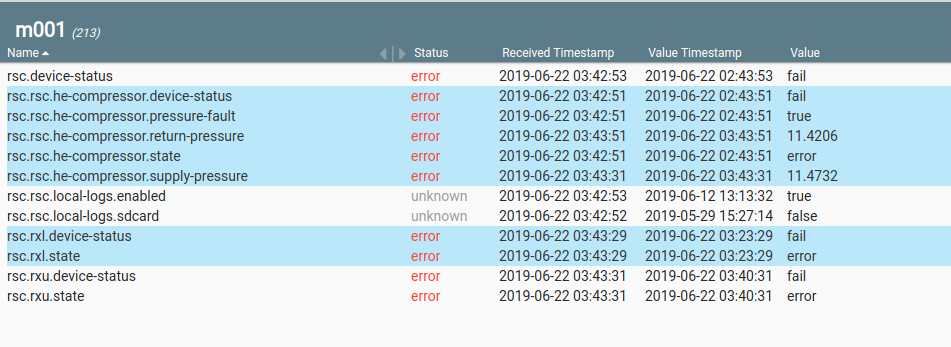
\includegraphics[scale=0.45]{Chapters/images/He1.png}
	
	%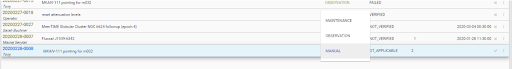
\includegraphics[resolution=100]{bur1.png}
	\caption{Receiver System Hellium presure errors}
	\label{fig:He1}
\end{figure}
\subsubsection{Helium compressor temperature fault}
\textbf{Figure}~\ref{fig:He2} shows the sensors that go into error when a temperature fault occurs.



\begin{figure}[!thb]
	\centering
	%\includegraphicsdpi{100}{}{bur1.png}     
	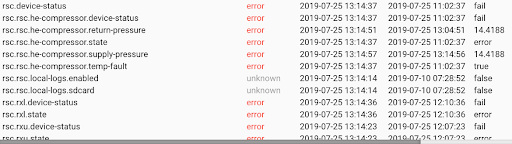
\includegraphics[scale=0.8]{Chapters/images/He2.png}
	
	%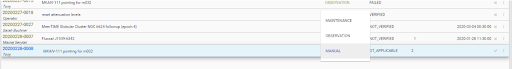
\includegraphics[resolution=100]{bur1.png}
	\caption{Receiver System temperature errors}
	\label{fig:He2}
\end{figure}
Note the only difference in sensors between the two faults mentioned above is the sensor indicating the type of fault:
\begin{lstlisting}[style=DOS]
rsc.rsc.he-compressor-pressure-fault (for pressure faults)
rsc.rsc.he-compressor-temp-fault (for temperature faults)
\end{lstlisting}

If one of these faults thus occur, report the issue as such (you don’t have to also report that the receivers are warm in a separate report, since helium compressor faults automatically cause receivers to warm up).

The following helium compressor sensors can be ignored (no action needed) when they go into error as they have no control value over the receivers and thus won’t affect observations in any manner:
\begin{lstlisting}[style=DOS]
rsc.rsc.he-compressor.temperature1
rsc.rsc.he-compressor.temperature2
\end{lstlisting}

\subsection{ Receivers System Debugging Tools}
We have debugging tools for the receivers systems which technicians use to predict failures and reporting of the receiver system status.  (You can either choose the “\file{rx\_daily}” folder to view the daily receiver reports or the “\file{rx\_monthly}” folder to view the monthly receiver reports). The tool is written in an ipython notebook and it is executed daily to provide daily reports. 

The following sensors can be ignored (no action needed as they are disabled and thus will show “unknown” status) as they have no control value over the receivers and thus won’t affect observations in any manner:
\begin{lstlisting}[style=DOS]
rsc.rsc.local-logs.enabled
rsc.rsc.local-logs.sdcard
\end{lstlisting}


Receiver Health by colour coding
Table 1

\section{Digitisers Checks and Setting up }




\section{Moving Skarabs}


\textbf{WARNING}:\textit{ do not try to move the skarabs right after stopping or starting a subarray. The SKARABs need a couple of minutes to restart. Otherwise, they will not be found by the script, and will be left behind on the unwanted cmc.}\\

\subsection{CMC IP addresses}
The IP addresses for different machines are:
\begin{itemize}


	\item[] \server{cmc1: 10.103.254.1} and name: \server{cmc1.cbf.mkat.karoo.kat.ac.za}
\item[] \server{cmc2: 10.103.254.3} and name: \server{cmc2.cbf.mkat.karoo.kat.ac.za}, 

\item[] You can use the IP addresses or hostnames interchangeably (whichever you prefer) 


\item[] The cbf\_support repository is on git. You can clone it from:\\
git clone \url{https://github.com/ska-sa/cbf_support}
\end{itemize}
\subsection{Check the number of SKARABS}
In order to check the number if SKARABS are available in the CMC use the following
commands on the obs machine before attempting to move them. There should be about 220(as at 2020-01-06, but more will come) if they were all moved. If there are less, wait a couple
of minutes for them to restart.

\begin{lstlisting}[style=DOS]
kcpcmd -t 10 -s cmc1.cbf.mkat.karoo.kat.ac.za:7147 resource-list | grep "up$" | wc -l
\end{lstlisting}
(this will give you the number of skarabs available on cmc1.) 
\begin{lstlisting}[style=DOS]
kcpcmd -t 10 -s cmc2.cbf.mkat.karoo.kat.ac.za:7147 resource-list | grep "up$" | wc -l
\end{lstlisting}
(this will give you the number of skarabs available on cmc2.) \\

\subsection{Moving SKARABS}
\begin{lstlisting}[style=DOS]
./usersnfs/cbf_support/./cmc_manage_skarabs.py -m cmc1 -a 5 6 7 8 9 10 11 12 13 14 15 16 17 18 -k cmc1 cmc2
\end{lstlisting}
\textbf{If moving to cmc2 use -m cmc2}:
\begin{lstlisting}[style=DOS]
./usersnfs/cbf_support/./cmc_manage_skarabs.py -m cmc2 -a 5 6 7 8 9 10 11 12 13 14 15 16 17 18  -k cmc1 cmc2
\end{lstlisting}




This will connect to all the switches, discover which skarabs are currently online on the various ports, and move them to the requested master controller (-m switch).



\section{Global Synchronisation}

This script seeks to synchronize all digitisers to the Digitiser Master Controller so that signal/data coming into the correlator is in sync and correlates. 
\begin{itemize}
\item{} Ensure epoch sync on all usable digitisers (all bands) is done for the day
\item{} In the GUI, verify that all subarrays are inactive
\end{itemize}

\section{Digitisers checks and setting up }
\section{Requesting which receptors have UHF-band digitisers}


\subsection{To check if profilers are on or off}
\subsubsection{To switch profilers off}
\subsubsection{To switch profilers on}
\subsection{To check which antenna belong to which proxy}
\section{AP Point Error Tiltmeters}
\subsection{SE tilt sensor measurements observations [if wind < 4 m/s]}
\subsection{Flights}



	